% file: 3-6-graph-decomposition/dfs-back-edge.tex

\documentclass[tikz]{standalone}
\usetikzlibrary{positioning}

\begin{document}
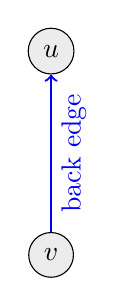
\begin{tikzpicture}[vertex/.style = {draw, circle, minimum size = 8pt},
  node distance = 2.0cm and 1.5cm,
  every edge/.style = {draw, thick}]
  \node (u) [vertex, fill = lightgray!30] {$u$};
  \node (v) [vertex, below = of u, fill = lightgray!30] {$v$};

  \path (v) edge[blue, ->] node[below, sloped] {back edge} (u);
\end{tikzpicture}
\end{document}
